\chapter{Svolgimento \emph{stage}}
\label{cap:svolgimentoStage}
In questo capitolo vengono descritte tutte le attività da me svolte durante lo \emph{stage}, divise nelle sezioni "Analisi", "Progettazione" e "Sviluppo software e documentale", in modo da fornire una panoramica chiara e strutturata del lavoro svolto, evidenziando il processo seguito e le competenze acquisite in ciascuna attività.\\
\section{Analisi}
\subsection{Requisiti}
I requisiti del mio \emph{stage}, derivanti in parte dalle dichiarazioni aziendali presenti nel documento "Progetto Formativo" generato all'inizio del suo svolgimento, e in parte conseguenza dell'analisi dei requisiti avvenuta in corrispondenza con la presenza di specifiche necessità progettuali, sono divisi in categorie:
\begin{enumerate}
	\item[O -]requisiti obbligatori, vincolanti in quanto obiettivi primari richiesti dall'azienda.
    \item[D -]requisiti desiderabili, non strettamente necessari ma dal riconoscibile valore aggiunto.
    \item[F -]requisiti facoltativi / opzionali, rappresentanti un valore aggiunto non strettamente competitivo.
\end{enumerate}

\begin{longtable}{|c|p{11cm}|}
\caption{Tabella dei requisiti progettuali.}
\label{tab:obiettiviProgettuali}\\
\hline \textbf{Codice} & \textbf{Descrizione}\\ \hline \endfirsthead
\hline \textbf{Codice} & \textbf{Descrizione}\\ \hline \endhead
\hline \endfoot
\hline \endlastfoot
\textbf{O1}    & Comprensione e mappatura delle funzionalità possibili tramite l'adozione dell'applicazione Microsoft Power Automate.\\
\hline O1.1  & Analisi approfondita riguardo ai flussi Power Automate ed individuazione delle caratteristiche, positive e negative, della sua adozione in azienda. Redazione di un documento dedicato.\\
\hline O1.2  & Sviluppo di almeno un flusso Power Automate.\\
\hline O1.3  & Produzione ed esposizione al \emph{tutor} aziendale e al \emph{team} di sviluppo di una presentazione riguardo ai risultati della mia analisi sull'adozione di Power Automate in azienda.\\
\hline \textbf{O2}  & Comprensione ed utilizzo della tecnologia Microsoft Power Apps e relative fasi di sviluppo collaborativo.\\
\hline O2.1  & Comprensione di Power Apps mediante lo svolgimento di attività di affiancamento con il \emph{team} di sviluppo fino al raggiungimento della comprensione dei metodi lavorativi e dei prodotti aziendali sviluppati con tale strumento.\\
\hline O2.2  & Identificazione e utilizzo di un metodo adatto allo sviluppo collaborativo di applicazioni Power Apps.\\
\hline O2.3  & Ottenimento di avanzamenti nello stato dei lavori di applicazioni aziendali realizzate con Power Apps.\\
\hline \textbf{O3}  & Individuazione ed implementazione di un efficace sistema di versionamento per progetti realizzati utilizzando tecnologie Power Automate e Power Apps\\
\hline \textbf{O4}  & Comprensione delle metodologie \gls{DevOps} e realizzazione della documentazione relativa alla sua applicabilità su tecnologie Power Automate e Power Apps.\\
\hline 
\hline \textbf{D1}  & Collaborazione con gli altri stagisti universitari e individuazione di soluzioni collaborative relative ai bisogni progettuali comuni.\\
\hline \textbf{D2}  & Realizzazione di PoC a supporto delle soluzioni individuate durante le fasi di ricerca.\\
\hline D2.1  & Realizzazione di PoC riguardo allo sviluppo di flussi Power Automate approvativi.\\
\hline D2.2  & Realizzazione di PoC riguardo all'integrazione tra flussi Power Automate ed elementi esterni tramite le chiamate \gls{http}.\\
\hline D2.3  & Realizzazione di PoC riguardo al processo \gls{DevOps} di \emph{build} su progetti realizzati con tecnologie Power Automate/Power Apps.\\
\hline D2.4  & Realizzazione di PoC riguardo al processo \gls{DevOps} di \emph{test} su progetti realizzati con tecnologie Power Automate/Power Apps.\\
\hline \textbf{D3}  & Esecuzione di \emph{meeting} e scambio di documenti con gli altri stagisti universitari al fine di comprendere l'applicabilità delle fasi di \gls{DevOps} in ambito \gls{Sistemi} \\
\hline 
\hline \textbf{F1}  & Esplorazione della tecnologia Angular mediante realizzazione di un progetto di \emph{test}\\
\hline \textbf{F2}  & Integrazione di un progetto Angular con le fasi di \gls{DevOps} mediante un \emph{server} Jenkins.\\
\hline \textbf{F3}  & Realizzazione ed esposizione di una presentazione finale, in collaborazione con gli altri stagisti, riguardo tutto il lavoro fatto durante lo \emph{stage}.\\
\end{longtable}

\subsection{Ambiente di lavoro}
Durante i primi giorni dello \emph{stage} sono stato introdotto all'ambiente di lavoro e alle tecnologie di comunicazione e collaborazione utilizzate.\\
Conseguentemente ho analizzato e utilizzato il sistema di messaggistica basato su Microsoft Teams e Outlook e ho compreso la struttura di condivisione dei dati, utilizzata in azienda, basata sullo strumento Microsoft SharePoint.
Esso è una piattaforma \emph{software} in grado di organizzare dati sottoforma di \emph{file} e strutture tabellari chiamate "Liste", al fine di gestire il materiale condiviso dall'azienda e dai singoli \emph{team} tramite un sistema di accessi e autorizzazioni.\\
Tramite questi strumenti ho studiato i documenti aziendali a me forniti in modo da comprendere i principali processi produttivi di Wintech.\\ 
Tali documenti comprendono i "Documenti di sviluppo sicuro" e includono:
\begin{itemize}
    \item Agile e SCRUM: descrizione delle metodologie Agile e SCRUM, spiegazione dei ruoli necessari e delle cerimonie previste. 
    \item Presentazione sviluppo sicuro: presentazione PowerPoint che descrive i processi aziendali atti a migliorare la qualità dei prodotti realizzati automatizzando fasi ripetitive e rispettando criteri di sicurezza. 
    \item Modelli di sviluppo sicuro: elenco dettagliato dei documenti di sviluppo sicuro i quali descrivono come applicare automazioni processuali (per esempio i processi di \emph{build} e \emph{deploy}) in modo sicuro e normato. 
    \item Politiche di sviluppo sicuro: strategie e normative aziendali definite al fine di garantire sicurezza e qualità nei processi e nel ciclo di vita del \emph{software}. 
    \item Piani di progetto degli altri stagisti: piani formativi degli altri due stagisti che nel mio stesso periodo hanno effettuato lo \emph{stage} universitario in Wintech. 
\end{itemize}
Relativamente a quest'ultimo punto, nei primi giorni ho approfondito il lavoro svolto dagli altri stagisti tramite appositi \emph{meeting} nei quali mi hanno descritto i risultati ottenuti fino a quel momento. Essi, avendo iniziato lo svolgimento del progetto circa una settimana prima, mi hanno esposto, mediante apposite presentazioni PowerPoint, le proprie ricerche riguardanti l'utilizzo dello strumento Git e dello studio avvenuto riguardo la possibilità di integrare tra loro gli strumenti Planner e Taiga. 

\subsection{Tecnologie oggetto di \emph{stage}}
Questa sottosezione descirve i metodi di apprendimento e le nozioni apprese durante la fase di analisi delle tecnologie su cui si basa la ricerca del mio progetto di \emph{stage}.\\
Dopo aver compreso le tecnologie e i principali processi aziendali, ho partecipato ad un \emph{meeting} con il \emph{tutor} aziendale al fine di discutere il mio progetto di \emph{stage}.\\
Gli obiettivi scaturiti da tale incontro sono stati: 
\begin{itemize}
    \item Autoapprendimento dello strumento Power Automate.
    \item Realizzazione di un PoC che testasse la possibilità di realizzare un flusso approvativo Power Automate. 
    \item Testare le funzionalità disponibili con le licenze di utilizzo \emph{standard}. 
\end{itemize}

\subsubsection*{Power Automate}
Ho pertanto studiato approfonditamente tali tecnologie con l'ausilio delle numerose guide e \emph{tutorial} offerti da Microsoft. 
Essi sono direttamente accessibili dalla \emph{home} di Power Automate e Power Apps e sono divisi in moduli testuali corredati da immagini, dalla durata e argomenti specifici. 

\begin{figure}[htbp] 
    \centering 
    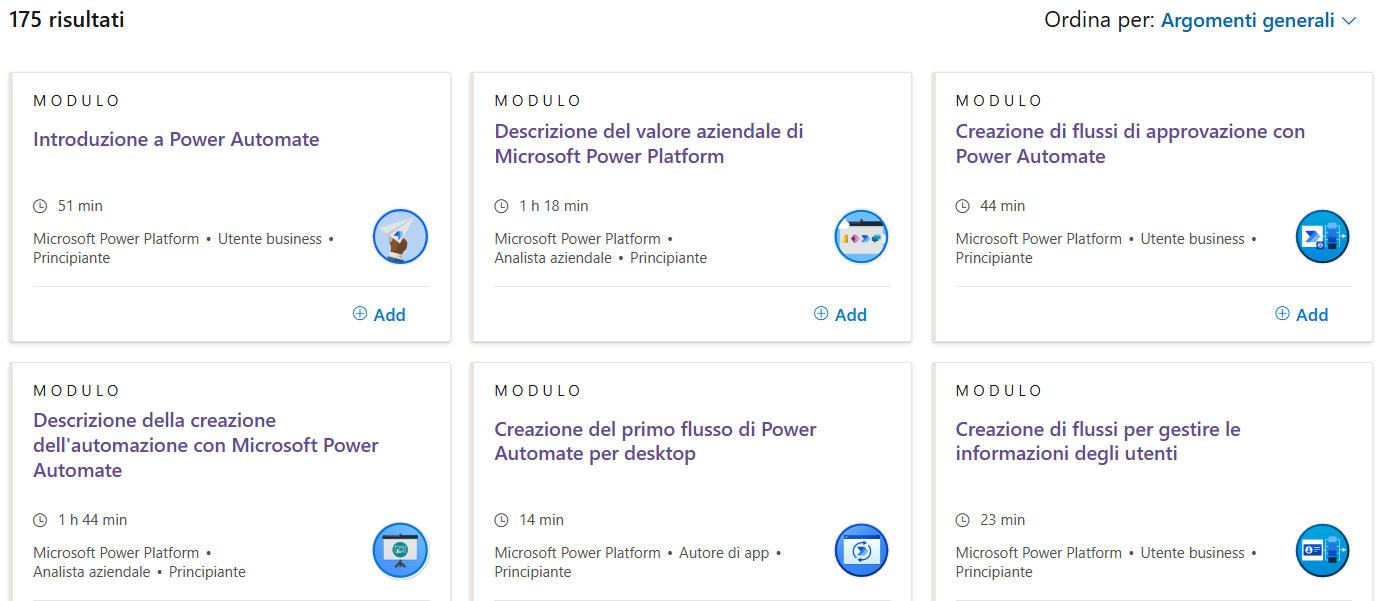
\includegraphics[width=1\columnwidth]{moduliPowerAutomate} 
    \caption{Moduli formativi per Power Automate.}
    \label{fig:moduliPowerAutomate}
    \vspace{1mm}
    Fonte: \url{https://learn.microsoft.com/it-it/training/browse/?products=power-automate}.
\end{figure}

\noindent Lo studio di tali moduli mi ha permesso di comprendere il funzionamento e le \emph{features} principali di Power Automate.
Esso è formato da una pagina \emph{web} che offre controllo sui flussi di automazione creati: è possibile modificarli e visualizzarne i dettagli, le esecuzioni e le statistiche. Inoltre, si possono creare dei nuovi flussi partendo da altri progetti pubblici, o a noi condivisi, e modelli offerti da Microsoft da adattare alle proprie esigenze.\\
La modifica di un flusso non avviene mediante la scrittura di codice tramite un linguaggio di programmazione, bensì tramite una composizione "a blocchi" personalizzabili collegati tra loro ciascuno avente proprietà e attributi definiti.\\
Essi sono selezionabili da una lista di blocchi relativi ciascuno a una funzionalità specifica di un servizio Microsoft.
Tali blocchi possono essere "Trigger" o "Azioni" ed entrambi sono necessari per la creazione e il funzionamento di un flusso.
In ogni flusso è presente uno e un solo Trigger il quale rappresenta il suo punto di partenza nonché la condizione che scaturisce la sua esecuzione.\\
Esistono tre tipologie principali di Trigger le quali determinano la tipologia stessa di ogni flusso:
\begin{itemize}
    \item Automatico: per esempio "SharePoint - Quando viene creato un elemento". 
    \item Istantaneo: per esempio "Attiva manualmente un flusso".
    \item Pianificato: per esempio "Ricorrenza", il quale attiva il flusso periodicamente.\\
\end{itemize}

\noindent Ad ogni Trigger possono essere collegate, in serie o in parallelo, una moltitudine di Azioni, ciascuna responsabile di uno specifico compito, per esempio sono presenti le azioni "Inizializza variabile", "Avvia e attendi un'approvazione", "Teams - Crea una chat" e "Outlook - Invia un messaggio di posta elettronica".\\
Sono inoltre presenti azioni dedicate alla gestione logica dei flussi come "Condizione" e "Do until". La prima rappresenta la struttura di controllo rappresentata nei classici linguaggi di programmazione con "if", responsabile della ramificazione dell'esecuzione del flusso in base a una condizione specifica.
La seconda rappresenta la struttura di controllo rappresentata nei classici linguaggi di programmazione con "Do while", responsabile della ripetizione condizionata di un insieme di azioni garantendone sempre la prima esecuzione.
\begin{figure}[htbp] 
    \centering 
    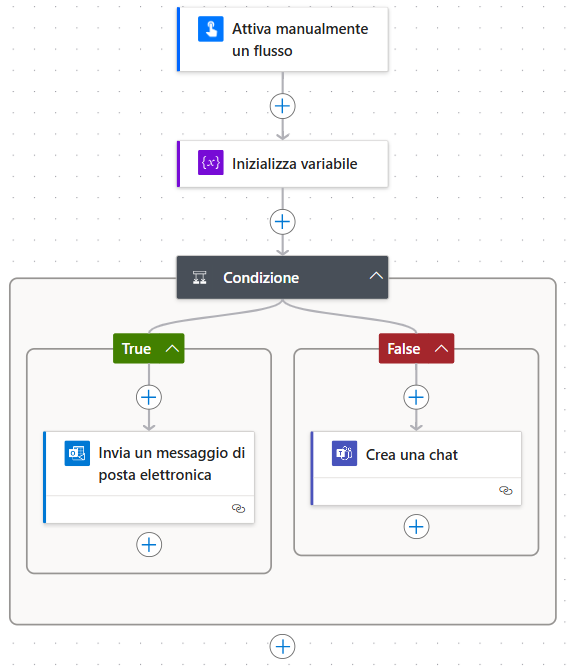
\includegraphics[width=0.6\columnwidth]{esempioFlusso} 
    \caption{Esempio di un flusso Power Automate istantaneo.}
    \label{fig:esempioFlusso}
\end{figure}
\newline \noindent Successivamente ho individuato, durante un meeting con il \emph{tutor} aziendale, la necessità di integrare i flussi Power Automate con il \emph{software} gestionale \hyperref[WOW]{WOW} e gli altri prodotti aziendali, al fine di poter integrare le funzionalità desiderate con libertà mantenendo coordinate le diverse parti del prodotto.\\
Sono emersi quindi due requisiti: il primo, utile per apprendere le tecnologie in oggetto, è relativo alla creazione di un flusso che automatizzi un processo approvativo (requisito D2.1).\\
Il secondo (requisito D2.2), più concreto e integrabile con i prodotti aziendali, si focalizza sull'applicazione ai flussi Power Automate di chiamate \gls{http}(Hypertext Transfer Protocol): in italiano "protocollo di trasferimento ipertestuale", è un protocollo di rete, ovvero un insieme di regole formalmente descritte che definiscono le modalità di comunicazione tra due o più apparecchiature elettroniche, usato come principale sistema per la trasmissione di informazioni sul \emph{web}.
\subsubsection*{Power Apps}
I flussi Power Automate portano grande vantaggio in termini di efficienza dei processi aziendali e possono aumentare il numero di funzionalità di un'applicazione.\\
Per questo motivo il loro utilizzo assume maggiore significato quando associato alla realizzazione di applicazioni Power Apps, le quali sono pensate per integrare nativamente i flussi creati.\\
Il metodo di apprendimento con cui ho analizzato e studiato Power Apps deriva non solo da attività individuali tramite i moduli didattici offerti da Microsoft nell'apposito sito \emph{web}, simili a quelli per Power Automate, ma soprattutto grazie alla collaborazione con un membro del \emph{team} di sviluppo che ho affiancato.\\
Egli è il responsabile in azienda di tutti i loro prodotti realizzati utilizzando le tecnologie oggetto del mio \emph{stage}, e assieme le abbiamo attentamente analizzate e modificate al fine di migliorarle ed applicarci le soluzioni da me individuate relativamente alle pratiche \gls{DevOps} richieste.\\
Power Apps offre la possibilità di creare nuove applicazioni e visionare quelle già create, o a noi condivise, con la possibilità di apportare modifiche.\\
È inoltre possibile visualizzare informazioni e statistiche relative a tutte le applicazioni in nostro possesso.\\
Il loro sviluppo non avviene esclusivamente mediante codice di programmazione bensì dall'utilizzo di componenti, \emph{standard} o \emph{custom}, che vengono manualmente posizionati sull'interfaccia, creando in questo modo una struttura gerarchica ad albero chiamata "Tree View".
\begin{figure}[htbp] 
    \centering 
    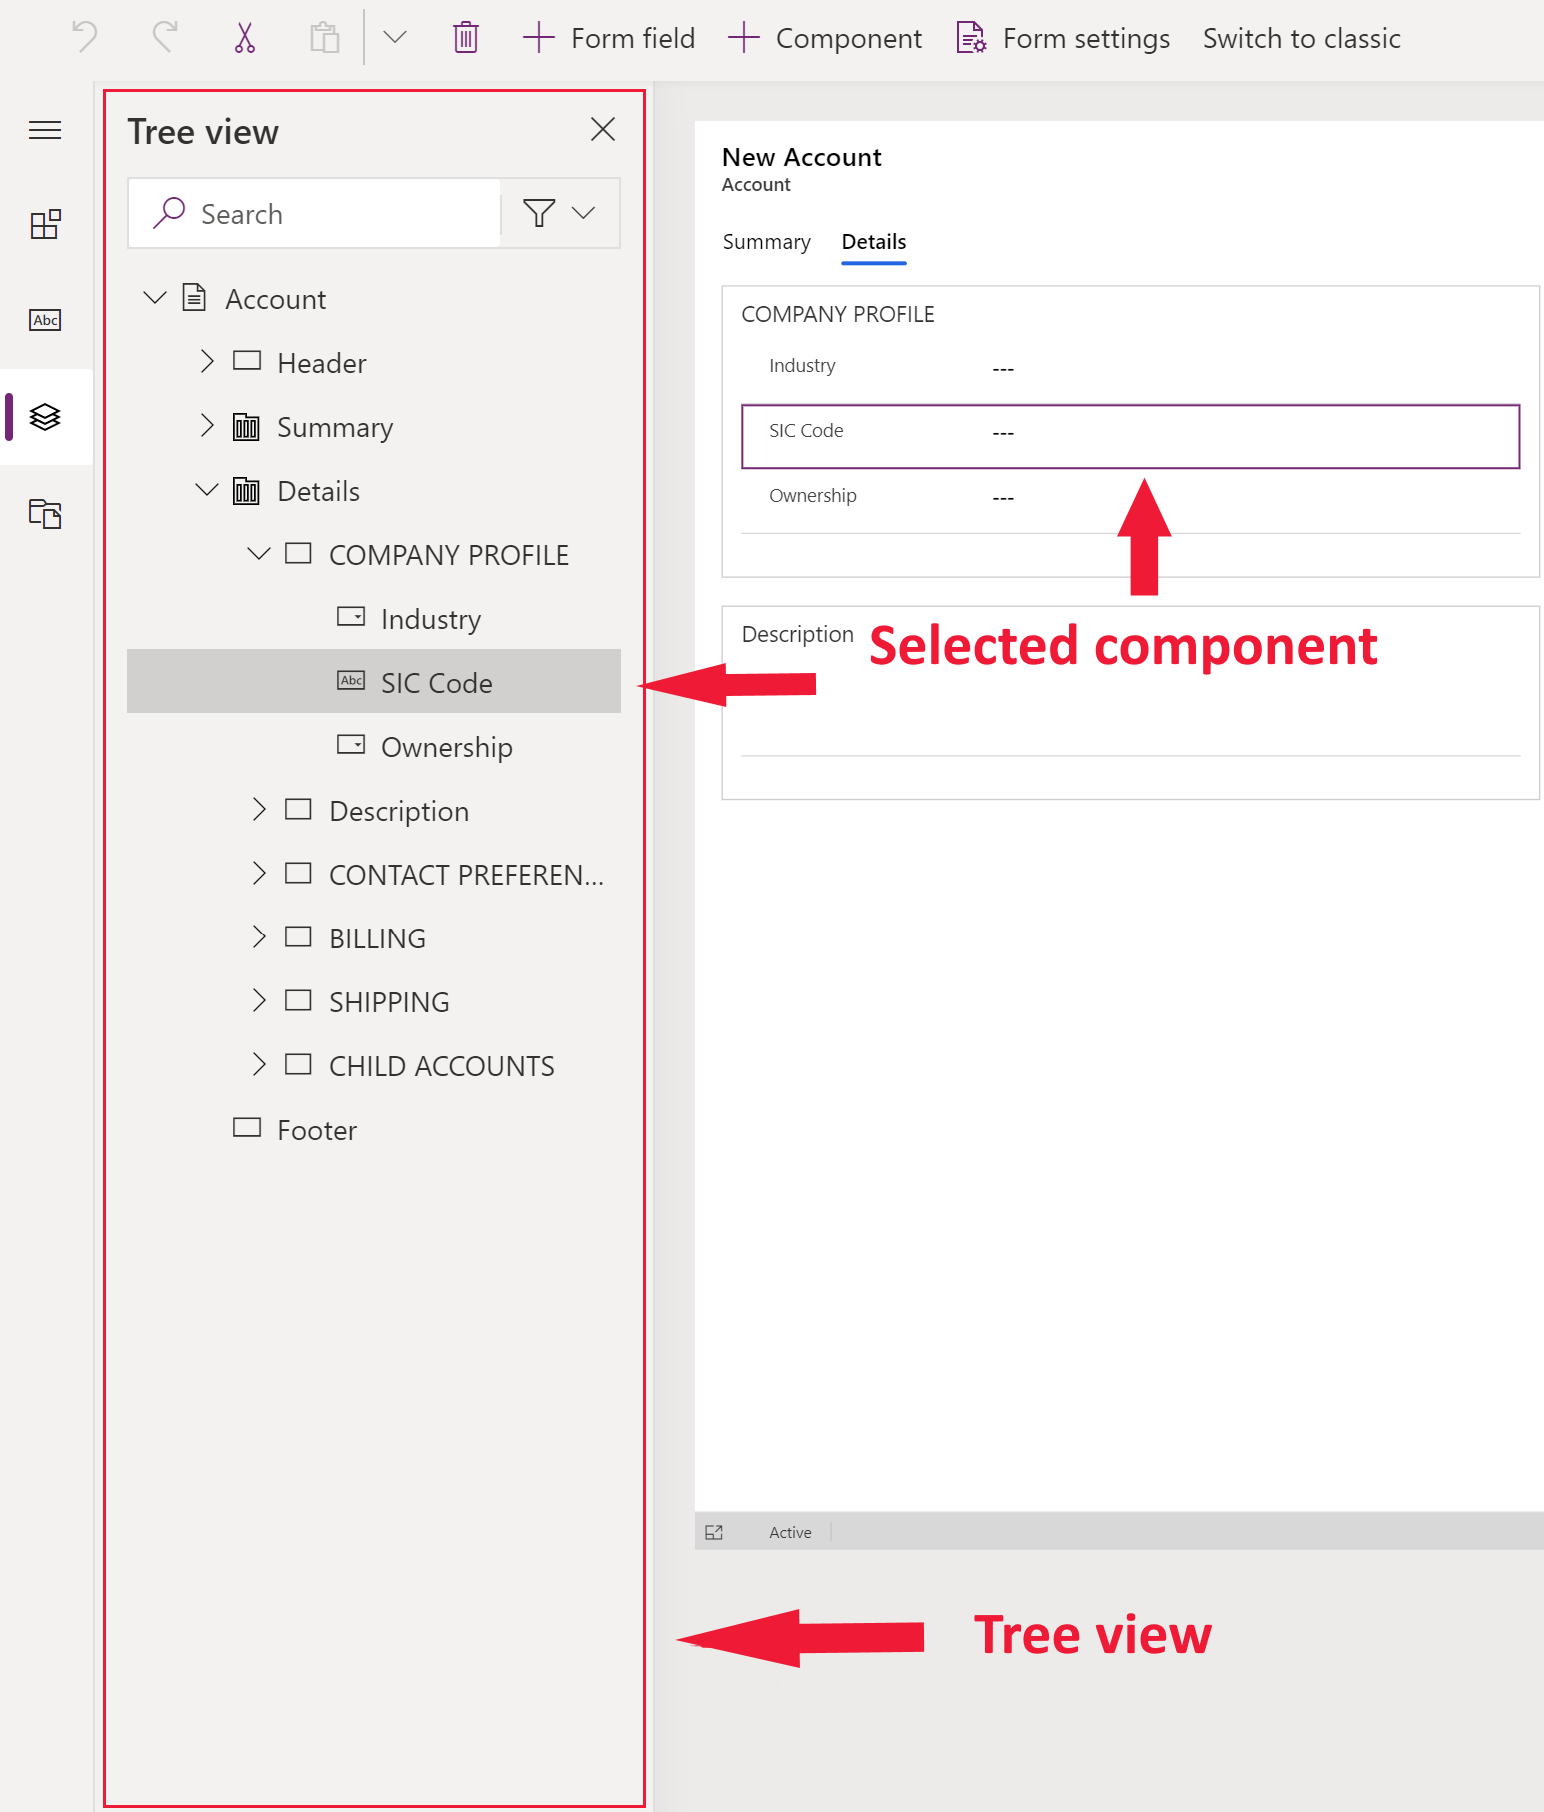
\includegraphics[width=0.6\columnwidth]{powerAppsTreeView} 
    \caption{Elemento Tree View per la gestione gerarchica dei componenti.}
    \label{fig:powerAppsTreeView}
    \vspace{1mm}
    Fonte: \url{https://learn.microsoft.com/en-us/power-apps/maker/model-driven-apps/using-tree-view-on-form}.
\end{figure}
\newline \noindent Al fine di modificare i parametri che lo compongono, ciascun componente può essere personalizzato tramite un'apposita finestra dell'interfaccia grafica.\\
Questo non comprende solo le peculiarità grafiche ma soprattutto il loro comportamento a seguito di azioni specifiche: per esempio è possibile creare un componente "Pulsante" e personalizzarne il campo "OnSelect" al fine di eseguire conseguentemente un flusso Power Automate e inviarne i dati di \emph{output} ad un altro componente.\\
Tali istruzioni vengono definite utilizzando Microsoft Power Fx, il quale rappresenta un linguaggio di programmazione dichiarativo, fortemente tipizzato e con uso limitato di codice, usato in Microsoft Power Platform.\\
Quest'ultima piattaforma include un insieme di strumenti e tecnologie, compresi Power Automate e Power Apps, pensati per offrire la possibilità di sviluppare prodotti \emph{software} con limitata necessità di scrivere, e conoscere, codice tramite linguaggi di programmazione.\\\\

\subsection{Tecnologie di supporto}
\subsubsection*{Jenkins}
Al fine di applicare le automazioni necessarie per adottare al \emph{software} le metodologie \gls{DevOps}, come richiesto dagli obiettivi di \emph{stage}, ho individuato lo strumento Jenkins in quanto esso rispecchia perfettamente le mie necessità ed è inoltre già conosciuto e applicato dal resto del \emph{team} di sviluppo, rappresentando quindi una tecnologia consolidata che non necessita di ulteriore formazione all'interno dell'azienda.\\
Ho appreso le conoscenze necessarie per studiare e utilizzare tale strumento in totale autonomia mediante la consultazione delle guide e del numeroso materiale presente \emph{online} comprese le pagine \emph{web} ufficiali di Jenkins con gli annessi video \emph{tutorial}.\\
Esso è uno strumento scritto in linguaggio di programmazione Java che viene eseguito all'interno di un \emph{web server} e offre la possibilità di creare, gestire, eseguire e monitorare dei progetti Jenkins chiamati "Job", potendone visionare e registrare i \emph{report} di \emph{output}.\\
Essi sono unità di lavoro configurabili che rappresentano un'attività o un progetto specifico che Jenkins esegue. Inoltre possono essere di diverso tipo ma tutti sono basati sull'esecuzione di uno \emph{script} o una \emph{pipeline} di automazione.\\
Una \emph{pipeline} Jenkins è una sequenza di fasi chiamate "Stage", eseguite in serie o in parallelo, responsabili di specifiche operazioni definite dall'utente, per esempio \emph{build}, \emph{test}, \emph{deploy}.\\
Esse possono essere definite tramite il linguaggio di programmazione Groovy oppure tramite l'interfaccia grafica di Jenkins.\\
Questo strumento permette dunque di fornire servizi di integrazione continua ed è indicato per l'applicazione di alcune fasi di \gls{DevOps} come Build e Test, il caricamento automatico dei \emph{file} sul \emph{repository} di versionamento desiderato e l'autenticazione automatica ai servizi Microsoft tramite comandi Power Platform CLI.\\
Quest'ultima è un'interfaccia a riga di comando che offre la possibiltà di eseguire un insieme di comandi specifici atti all'autenticazione e alla gestione degli ambienti e delle Microsoft Solutions.\\
\begin{figure}[htbp] 
    \centering 
    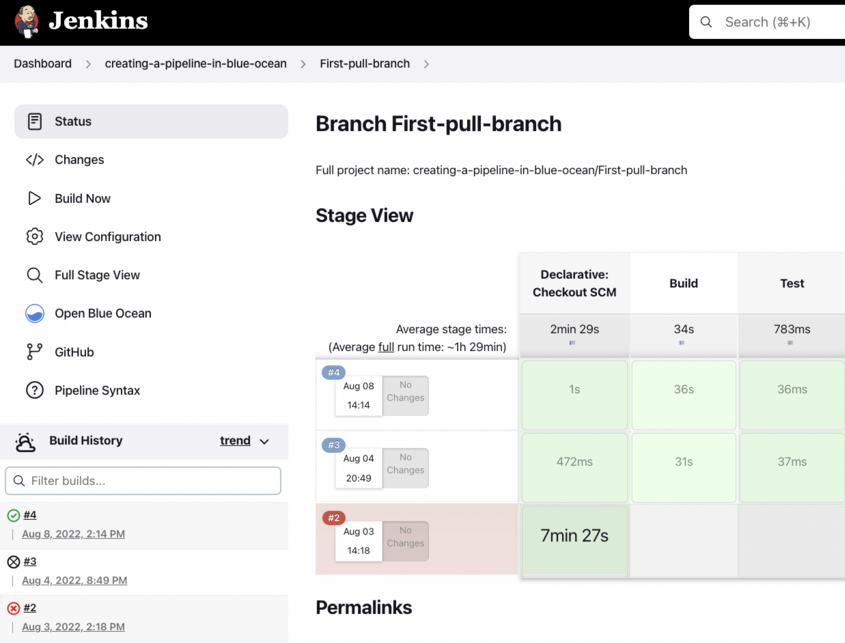
\includegraphics[width=0.9\columnwidth]{esempioJenkins} 
    \caption{Esempio interfaccia di Jenkins.}
    \label{fig:esempioJenkins}
    \vspace{1mm}
    Fonte: \url{https://commons.wikimedia.org/wiki/File:Updated-jenkins-view.png}.
\end{figure}

\newpage \subsubsection*{Microsoft Solutions}
Un'ulteriore oggetto di analisi e studio è stato l'utilizzo e la comprensione delle Microsoft Solutions. Esse fanno parte della \emph{suite} Microsoft Power Platform e sono degli strumenti che servono a contenere tutti i flussi Power Automate e applicazioni Power Apps corrispondenti a uno stesso progetto, in modo da poterli sviluppare e distribuire in maniera organizzata e centralizzata.\\
Esistono due tipi di Soluzioni: 
\begin{itemize}
    \item Gestite: destinate prevalentemente per gli ambienti di produzione e \emph{test}, non permettono la modifica degli elementi al suo interno. Per generare una Soluzione gestita è necessario esportare una soluzione non gestita.
    \item Non gestite: destinate prevalentemente per gli ambienti di sviluppo, permettono la modifica degli elementi al suo interno e la sua esportazione.
\end{itemize}
A differenza delle tecnologie precedentemente descritte, le Microsoft Solution non erano materia già affrontata in azienda, per cui il loro apprendimento è avvenuto in maniera totalmente autonoma mediante la documentazione presente nei siti \emph{web} Microsoft dedicati.\\
Le Soluzioni preservano i loro dati, e quelli degli elementi in esse contenuti, nel sistema di archiviazione Microsoft Dataverse che funge da \emph{database} centralizzato per applicazioni sviluppate con la Power Platform.\\
Tale adozione permette di usufruire di funzionalità altrimenti assenti.
Le conseguenze del loro utilizzo e le motivazioni che mi hanno portato ad utilizzare questa tecnologia sono materia di discussione presente nella sezione \hyperref[progettazioneSolutions]{Adozione delle Microsoft Solutions}.\\

\subsection{DevOps}
Prima di poter progettare una soluzione applicativa al fine di applicare le fasi di \gls{DevOps} a progetti realizzati con Power Automate e Power Apps, ho analizzato e compreso quali fossero le implicazioni di ogni \emph{step}.\\
Ho approfondito tale pratica soprattutto studiando gli approfondimenti presenti sul sito \emph{web} di Atlassian, nota compagnia di \emph{software enterprise}, e dalla teoria sul ciclo di vita del \emph{software} e sulle metodologie di automazione dei processi aziendali appresa durante il percorso di studi universitario.\\
Ho inoltre studiato i documenti di sviluppo sicuro aziendali, nei quali sono presenti delle linee guida su come adottare il \gls{DevOps} in Wintech.\\
Le sue fasi sono:
\subsubsection*{Plan}
Essendo la fase iniziale del ciclo, ha lo scopo di definire i requisiti, pianificare il ciclo di vita del progetto e identificarne le metodologie di lavoro. Adottando una metodologa iterativa, è consono che la pianificazione e le conseguenti fasi successive, possano subire modifiche rispetto alle precedenti pianificazioni.

\subsubsection*{Code}
Dopo aver compreso cosa e come soddisfare i requisiti progettuali, vengono sviluppate le soluzioni individuate seguendo le metodologie e le norme definite in fase Plan.\\
Essendo il progetto di \emph{stage} basato su tecnologie non sviluppabili tramite strumenti tradizionali, come IDE non proprietari e linguaggi di programmazione consolidati, l'analisi della fase Code è stata necessaria per comprendere le funzionalità disponibili agli utenti al fine di sviluppare tali prodotti.\\
È compresa in questa fase anche la ricerca avvenuta al fine di individuare le metodologie e gli strumenti adatti a sviluppare progetti con le tecnologie in oggetto in maniera collaborativa e adottando un efficace metodo di versionamento.\\
Questo ha necessitato di uno studio sullo strumento Git, già ampiamente affrontato durante il percorso di studi universitari.\\
Infine, è compresa nella fase Code anche l'attività di analisi statica del codice, la quale supporta le fasi di sviluppo identificando e segnalando eventuali errori nel codice sorgente senza la necessità di eseguirlo.

\subsubsection*{Build}
Fase relativa alla creazione dei pacchetti e dei \emph{file} eseguibili costruiti partendo dal codice sorgente prodotto nella fase precedente.\\
Il risultato di questa operazione rappresenta il prodotto sul quale verranno effettuati i \emph{test} e le verifiche necessarie. 

\subsubsection*{Test}
Ottenuto l'artefatto generato dalla fase Build, esso può essere testato mediante l'utilizzo di svariati strumenti appositi.\\
Essi comprendono diversi tipi di \emph{test} dinamici: 
\begin{itemize}
    \item Test di unità: verifica che le singole unità di codice, per esempio funzioni, metodi o classi, funzionino come previsto.
    \item Test di integrazione: verifica che più parti di codice o servizi interagiscano tra loro correttamente.
    \item Test di carico: verifica il comportamento del sistema sotto carico normale ed elevato.
    \item Test di sicurezza: individua le eventuali vulnerabilità o minacce di sicurezza presenti nel sistema. 
\end{itemize}
Durante le fasi analitiche del mio \emph{stage}, ha avuto molta rilevanza lo studio sui metodi nativi ed esterni applicabili ai flussi Power Automate e alle applicazioni Power Apps al fine di applicare \emph{test}. 

\subsubsection*{Release}
Quando il prodotto è stato creato e testato, esso è considerato pronto per essere reso disponibile ai clienti, e viene quindi rilasciato identificandone una versione specifica.

\subsubsection*{Deploy}
Una versione rilasciata del prodotto viene distribuita nello specifico ambiente di produzione in cui gli utenti finali lo utilizzeranno, garantendone il corretto funzionamento.

\subsubsection*{Operate}
La gestione e il funzionamento dell'applicazione in produzione viene garantita tramite attività come l'amministrazione e la manutenzione dei \emph{server} e la risoluzione dei problemi. 

\subsubsection*{Monitor}
Al fine di garantire affidabilità e buone prestazioni del sistema distribuito, il suo comportamento viene osservato tramite strumenti che ne raccolgono e analizzano i dati. 
Vengono inoltre raccolti i \emph{feedback} degli utenti finali e dei clienti al fine di migliorare la qualità del prodotto. 

\subsection{Analisi delle applicazioni aziendali}
Il \emph{focus} principale dello \emph{stage} è compiere un'analisi sulle tecnologie al fine di raggiungere gli obiettivi riguardanti la ricerca sull'effettiva applicabilità delle pratiche di \gls{DevOps} ai progetti realizzati con Power Automate e Power Apps.
È stato però fin da subito definito che avrei alternato tali attività con fasi di sviluppo su applicazioni aziendali al fine di approfondire la conoscenza delle tecnologie in oggetto e di diventare operativo in modo più efficace.\\
Insieme al membro del \emph{team} di sviluppo responsabile per la realizzazione delle applicazioni Power Apps e dei flussi Power Automate aziendali, ho affrontato problemi di sviluppo di vario genere in funzione delle necessità del momento, potendo analizzare diversi prodotti aziendali.\\
Le effettive attività di programmazione svolte su queste applicazioni sono presenti nella sezione \hyperref[sviluppoApplicazioni]{Sviluppo di applicazioni aziendali}.\\
I principali prodotti su cui abbiamo collaborativamente lavorato sono:
\subsubsection*{Report di visita}
Principale applicazione su cui ho lavorato e con cui ho svolto attività di analisi al fine di comprendere le tecnologie utilizzate. Essa ha l'obiettivo di offrire la possibilità ad un dipendente dell'azienda, il quale dovesse trovarsi nella sede di un cliente, di registrare e condividere con i colleghi, in un ambiente condiviso, un \emph{report} della visita al fine di tracciare l'esperienza con il cliente.\\
Essa offre quindi la possibilità di: 
\begin{itemize}
    \item Ricercare e selezionare una specifica azienda visualizzabile in un'apposita lista a schermo 
    \item Visualizzare le sedi e le filiali dell'azienda selezionata 
    \item Visualizzare le informazioni anagrafiche dei contatti dell'azienda selezionata  
    \item Visualizzare i \emph{report} di visita già creati come bozza  
    \item Modificare eventuali bozze selezionate 
    \item Creare un nuovo documento inserendo in un apposito \emph{form} i dati relativi all'operatore, al cliente e alla visita specifica 
    \item Salvare tale \emph{report} come bozza o come documento definitivo
    \item Caricare automaticamente i dati generati nel \emph{database} aziendale 
\end{itemize}
\begin{figure}[htbp] 
    \centering 
    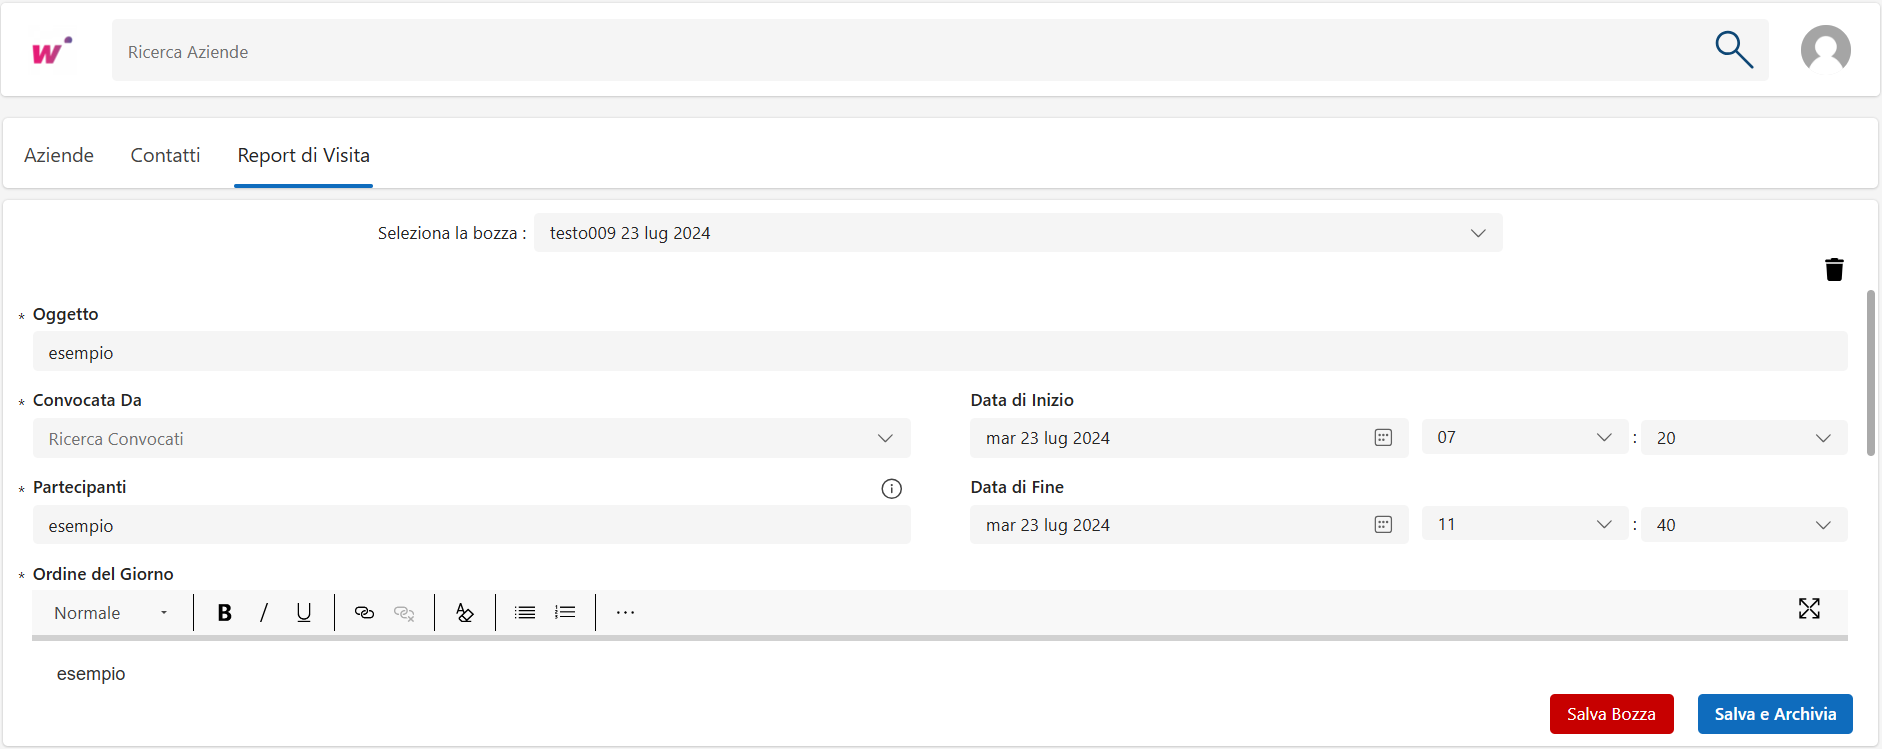
\includegraphics[width=1\columnwidth]{RDV} 
    \caption{Interfaccia grafica di Report di visita.}
    \label{fig:RDV}
\end{figure}

\subsubsection*{Registro accessi}
Applicazione realizzata al fine di gestire agevolmente i \emph{check-in} e \emph{check-out} lavorativi del personale.\\
Le funzionalità presenti sono: 
\begin{itemize}
    \item Identificazione del dipendente
    \item Selezione della sede, compresa la possibilità di selezionare lo \emph{smart working} o lavoro fuorisede 
    \item Selezione del \emph{check-in} 
    \item Visualizzazione di errore in caso di \emph{check-in} in mancanza del precedente \emph{check-out} 
    \item Selezione del \emph{check-out} 
    \item Visualizzazione di errore in caso di \emph{check-out} in mancanza del precedente \emph{check-in} 
    \item Visualizzazione di tutti i propri \emph{check-in} e \emph{check-out} 
\end{itemize}

\subsubsection*{Non conformità}
Nel momento in cui ho svolto lo \emph{stage}, questa applicazione era nelle sue prime fasi di sviluppo e le sue funzionalità non erano state ancora definite pienamente.\\
I suoi obiettivi sono quelli di creare e gestire un flusso approvativo a più \emph{step}, dove per ogni fase vengono notificati i corrispondenti incaricati, ai quali viene richiesta la compilazione di \emph{form} relativi alla non conformità di un prodotto e alle conseguenti azioni da intraprendere.\\

\subsection{Angular}
Gli ultimi requisiti emersi durante lo svolgimento dello \emph{stage} sono quelli relativi allo studio e all'applicazione di alcune fasi di \gls{DevOps} a progetti realizzati con lo strumento Angular.\\
Esso è un \emph{framework} per la realizzazione di applicazioni \emph{web} tramite il linguaggio di programmazione TypeScript e rappresenta una delle principali tecnologie usate dai \emph{team} di sviluppo di Wintech.\\
È per questo motivo che, nel momento in cui ho terminato le attività previste per il mio \emph{stage} con alcuni giorni di anticipo, mi è stato affidato il compito di studiare e provare ad utilizzare le stesse loro tecnologie e metodologie di lavoro al fine di comprenderle al meglio ed integrarmi maggiormente nell'ambiente lavorativo.\\
Tramite il sito \emph{web} ufficiale di Angular, ho seguito le guide fornite in modo da apprenderne le basi e poter realizzare quanto richiesto soddisfacendo i requisiti assegnati.\\

\section{Progettazione}
%In questa sezione sono presenti tutte le attività di progettazione da me svolte e il suo scopo è descrivere le modalità con cui ho individuato le soluzioni ai bisogni progettuali in modo da soddisfarne i requisiti.
\subsection{\emph{Scope} di Power Automate e Power Apps}
A seguito dell'analisi avvenuta sulle tecnologie oggetto di \emph{stage} è stato possibile identificare il compito che Power Automate e Power Apps devono avere all'interno di un progetto. 
Esse sono infatti tecnologie pensate per sviluppare in maniera rapida soluzioni relativamente semplici. Nel momento in cui ci fosse la necessità di applicare logiche molto complesse o l'integrazione con servizi esterni dalla \emph{suite} Microsoft, tali strumenti non sono più ideali in quanto si incomberebbe in numerosi vincoli tecnologici.
Questo è un fattore importante da considerare nelle fasi di progettazione di un progetto.\\

\subsection{Individuazione delle soluzioni tecnologiche}
In questa sottosezione vengono esplicitate le motivazioni che mi hanno portato a identificare determinate soluzioni al fine di soddisfare i requisiti compresi in fase di analisi.

\subsubsection*{Adozione delle Microsoft Solutions}
\label{progettazioneSolutions}
L'adozione delle Soluzioni, essendo esse basate sul sistema di archiviazione Dataverse, comporta la possibilità aggiuntiva di poter visionare la "Version history" dei flussi Power Automate. Tale funzionalità è in grado di ripristinare specifiche versioni precedenti dei flussi, agevolando le fasi di sviluppo.
\begin{figure}[htbp] 
    \centering 
    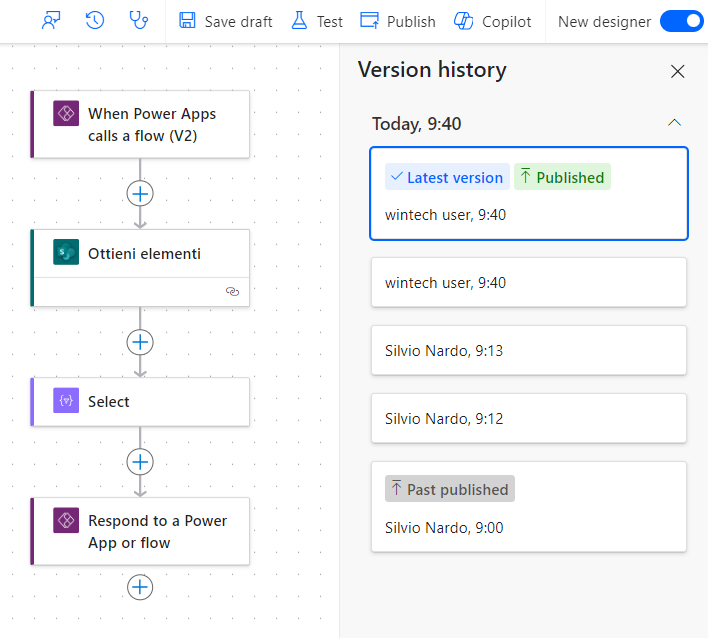
\includegraphics[width=0.8\columnwidth]{versionHistory} 
    \caption{Funzionalità Version history nei flussi Power Automate.}
    \label{fig:versionHistory}
\end{figure}
\newline \noindent Inoltre, essendo i componenti di una Soluzione contenuti in un unico pacchetto esportabile, la gestione dei progetti così organizzati risulta più agevole, soprattutto nelle fasi Build, Code e Deploy. 

\subsubsection*{Job Jenkins}
Riguardo alla scelta del tipo di Job da adottare in Jenkins, è stato individuato il "Multibranch Pipeline Job". Esso permette di collegare un \emph{repository} Git e ha la possibilità di gestire automaticamente una \emph{pipeline} indipendente, contenuta in un apposito \emph{file} chiamato "Jenkinsfile", per ogni \emph{branch}.
Tale Job ha inoltre la possibilità di eseguire automaticamente i Jenkinsfile corrispondenti solo ai \emph{branch} in cui è avvenuta una modifica, rendendo questo strumento ideale per la gestione di progetti Git.\\

\subsection{Soluzioni individuate per le fasi DevOps}
\subsubsection*{Plan}
Come strumenti identificati per la pianificazione delle attività sono stati utilizzati Planner e Taiga.
Essi permettono di categorizzare tutte le attività da assegnare al \emph{team} di sviluppo tramite \emph{tag} e contenitori specifici, i quali definiscono lo stato di avanzamento dei lavori.\\
Nello specifico, Planner viene utilizzato solo dal responsabile di progetto e serve a tenere traccia dei casi d'uso, mentre Taiga si occupa di tracciare i \emph{task} più specifici assegnati ai membri del \emph{team}, il quale si occupa di organizzarli.

\subsubsection*{Code}
Il versionamento di tutte le parti dei progetti realizzati con Power Apps e Power Automate è avvenuto in un singolo \emph{repository} Git in modo da garantire una migliore organizzazione dei dati e facilità di ripristino di specifiche versioni.\\
Per il lavoro collaborativo è stata individuata la \emph{feature} che integra il collegamento ad un \emph{repository} Git con Power Apps e permette di fare \emph{commit} e \emph{push} automaticamente.\\
Il \emph{repository} è diviso nei \emph{branch} "Main", per le versioni funzionanti e stabili del prodotto, "Develop", per il prodotto ancora in fase di sviluppo, e diversi \emph{feature branch} utilizzati dai singoli sviluppatori per apportare modifiche limitate a singole funzioni.\\
Per applicare a tali progetti l'analisi statica del codice, ho individuato come soluzione l'utilizzo degli strumenti nativi offerti da Microsoft:
\begin{itemize}
    \item Verifica flusso: permette l'esecuzione di un controllo sul codice e la visualizzazione di errori sul flusso come i campi obbligatori mancanti, gli \emph{input} non validi o i problemi legati alle licenze. 
    \item Verifica app: permette l'esecuzione di un controllo sul codice e la visualizzazione di errori sull'applicazione come formule Fx non valide, problemi di accessibilità o problemi legati alle origini dati. 
    \item Verifica soluzione: più dettagliata delle precedenti, permette l'esecuzione di un controllo sul codice e la visualizzazione di errori sui componenti della Soluzione.
\end{itemize}
\begin{figure}[htbp] 
    \centering 
    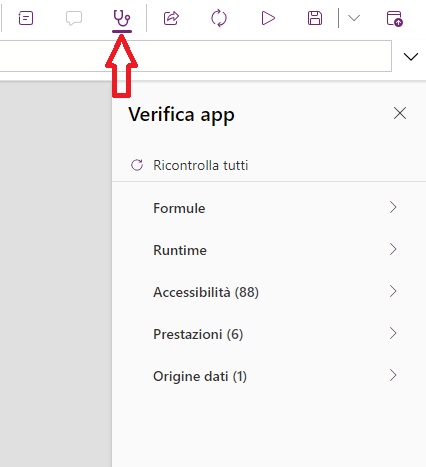
\includegraphics[width=0.6\columnwidth]{verificaApp} 
    \caption{Funzionalità Verifica App nelle applicazioni Power Apps.}
    \label{fig:verificaApp}
\end{figure}

\noindent Gli strumenti di analisi statica esterni non sono stati utilizzati poiché, a seguito di \emph{test} esplorativi e attività di ricerca in merito, è emersa l'eccessiva difficoltà nell'integrazione di qualsiasi strumento non offerto da Microsoft, ai \emph{file} generati dai flussi Power Apps e alle applicazioni Power Automate. 

\subsubsection*{Build}
I \emph{file} generati da Power Automate e Power Apps al fine di rappresentare i flussi e le applicazioni create nelle rispettive interfacce di sviluppo, sono rappresentati da un pacchetto compresso ZIP contenente i \emph{file} generati automaticamente da tali programmi.\\
Essi sono principalmente di tipo JSON, e .msapp e possiedono una struttura di difficile comprensione, pertanto non sono pensati per uno sviluppo manuale diretto.\\
Le Microsoft Solution sono rappresentate dai \emph{file} corrispondenti a quelli dei flussi e delle applicazioni in esse contenuti e nessuno di questi componenti possiede un \emph{file} eseguibile.\\
Come metodo per l'esecuzione della fase Build automatica, ho individuato i comandi forniti dalla Power Platform CLI, automatizzati da un Job Jenkins, al fine di esportare i pacchetti relativi alle Soluzioni desiderate. 

\subsubsection*{Test}
A causa della natura dei pacchetti di dati generati con la fase Build è emerso, similmente all'analisi statica del codice, la necessità di utilizzare principalmente gli strumenti nativi forniti da Microsoft per eseguire \emph{test} dinamici.\\
Per i flussi Power Automate è disponibile la funzione "Test" presente nell'interfaccia grafica di sviluppo.\\
Essa permette l'esecuzione del flusso e la visione dei suoi risultati compresi gli \emph{input} e \emph{output} di ogni azione e il loro tempo di esecuzione. 
Inoltre, in caso di errore, sono fornite le relative informazioni. 
\begin{figure}[htbp] 
    \centering 
    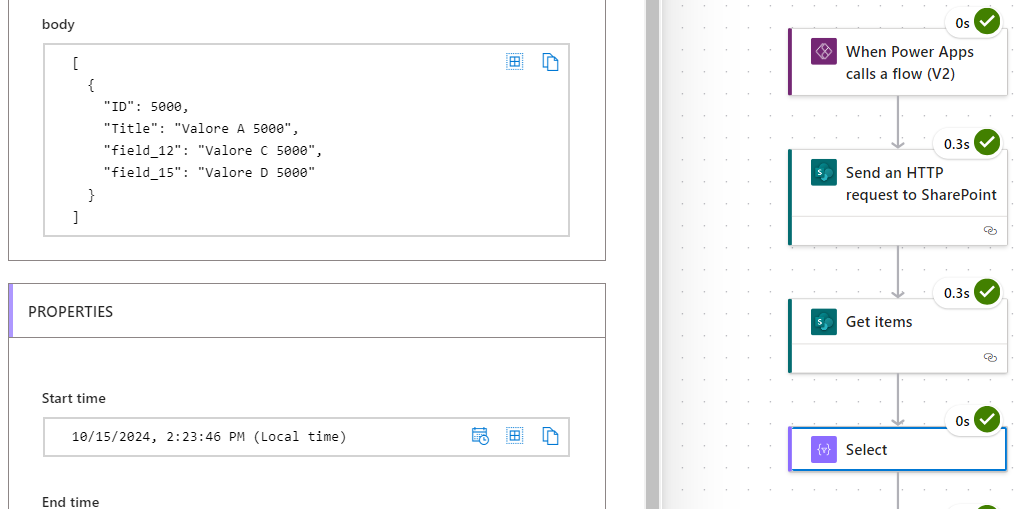
\includegraphics[width=1\columnwidth]{testFlusso} 
    \caption{Funzionalità Test nei flussi Power Automate.}
    \label{fig:testFlusso}
\end{figure}

\newpage \noindent Per eseguire \emph{test} esclusivamente su una specifica parte di un flusso Power Automate, simulando il comportamento delle azioni ad essa connesse, è disponibile la funzione "Static Result".\\
Essa permette un maggiore controllo sull'esecuzione del flusso durante i \emph{test} e l'azzeramento dei tempi di esecuzione di azioni che non rappresentano il suo \emph{focus}.\\
È inoltre stata individuata la possibilità di utilizzare i Trigger e le Azioni Power Automate legate all'utilizzo delle chiamate \gls{http}, al fine di estrapolare i dati di \emph{output} di un flusso ed elaborarli in uno \emph{script} esterno realizzato con l'ambiente Node.js, il quale sfrutta il linguaggio JavaScript. Maggiori informazioni su quanto sviluppato per questa soluzione sono presenti nella parte \hyperref[testProgrammazione]{Test} della sottosezione \hyperref[Sviluppo DevOps]{Sviluppo DevOps}.\\\\
Per quanto concerne i \emph{test} su applicazioni Power Apps, sono presenti diversi strumenti nativi per verificare la loro corretta esecuzione.\\
"Test studio" è uno strumento che permette di eseguire l'applicazione e registrare tutte le azioni intraprese dall'utente (o definite manualmente), al fine di generare uno \emph{script} di \emph{test} che possa ripetere tali azioni e fornire un riscontro.\\
Attualmente l'utilizzo di Test studio non è conveniente a causa del numero considerevole di limitazioni:
il suo funzionamento è limitato solo a componenti "classici", ovvero una lista di componenti presenti su Power Apps prima dell'arrivo dei componenti "moderni".\\
Esclude inoltre l'uso di componenti \emph{custom} e non è compatibile con l'integrazione nativa tra Power Apps e Git.\\\\
Per questi motivi la metodologia identificata per permettere il \emph{testing} ad applicazioni Power Apps è la funzionalità "Visualizza l'anteprima dell'app", con la quale è possibile eseguirla e verificarne il corretto funzionamento.\\
Nel caso in cui si verificassero degli errori durante tale operazione, i loro dettagli possono essere visualizzati. 

\subsubsection*{Release}
La strategia identificata per definire i rilasci è l'assegnazione di specifici \emph{tag} alfanumerici ai \emph{commit} nel \emph{repository} Git.\\
Tale codice è composto dalla lettera "v" seguita da tre cifre separate da un carattere ".", per esempio "v1.0.0".\\
Il criterio di avanzamento delle cifre è: 
\begin{itemize}
    \item Avanzamento della prima cifra: sono avvenute modifiche architetturali che alterano significativamente le funzionalità previste ad alto livello.\\
    Esempio: sostituzione di una tecnologia fondamentale per il funzionamento di un programma o cambiamento radicale dei casi d'uso individuati.  
    \item Avanzamento della seconda cifra: sono avvenute modifiche che alterano le funzionalità previste ad alto livello o ne aggiungono di nuove.\\
    Esempio: modifiche che soddisfano i requisiti di un caso d'uso non ancora risolto, aggiunta di classi in uno \emph{script} che alterano il comportamento precedente del programma, aggiunta di una nuova scheda di un'applicazione.
    \item Avanzamento della terza cifra: sono avvenute modifiche che non alterano significativamente le funzionalità previste ad alto livello.\\
    Esempio: \emph{Bug fix}, sostituzione di un componente di un'applicazione al fine di ottenere il medesimo risultato precedentemente atteso. 
\end{itemize}

\subsubsection*{Deploy}
Power Apps, Power Automate e le Micorsoft Solutions permettono non solo di esportare i pacchetti relativi ai propri progetti, ma anche di importarne di altri.\\
In tale funzione ho individuato il metodo per distribuire i prodotti negli ambienti di produzione. 

\subsubsection*{Operate}
L'operatività delle soluzioni implementate viene monitorata tramite il \emph{feedback} fornito dal cliente.\\
Nel caso in cui si verificasse un problema con tale prodotto, viene fornita immediato supporto al fine di soddisfare nuovamente le attese.\\
Nel caso in cui il problema riscontrato fosse molto problematico, il sistema di versionamento definito permette il ripristino del prodotto ad una precedente versione stabile. 

\subsubsection*{Monitor}
Il monitoraggio dei \emph{report} Jenkins, delle esecuzioni dei flussi Power Automate e delle esecuzioni delle applicazioni Power Apps, sono nativamente forniti dai rispettivi servizi. Tramite le interfacce disponibili è possibile vedere le informazioni sufficienti ad identificare eventuali problemi e "colli di bottiglia".
\begin{figure}[htbp] 
    \centering 
    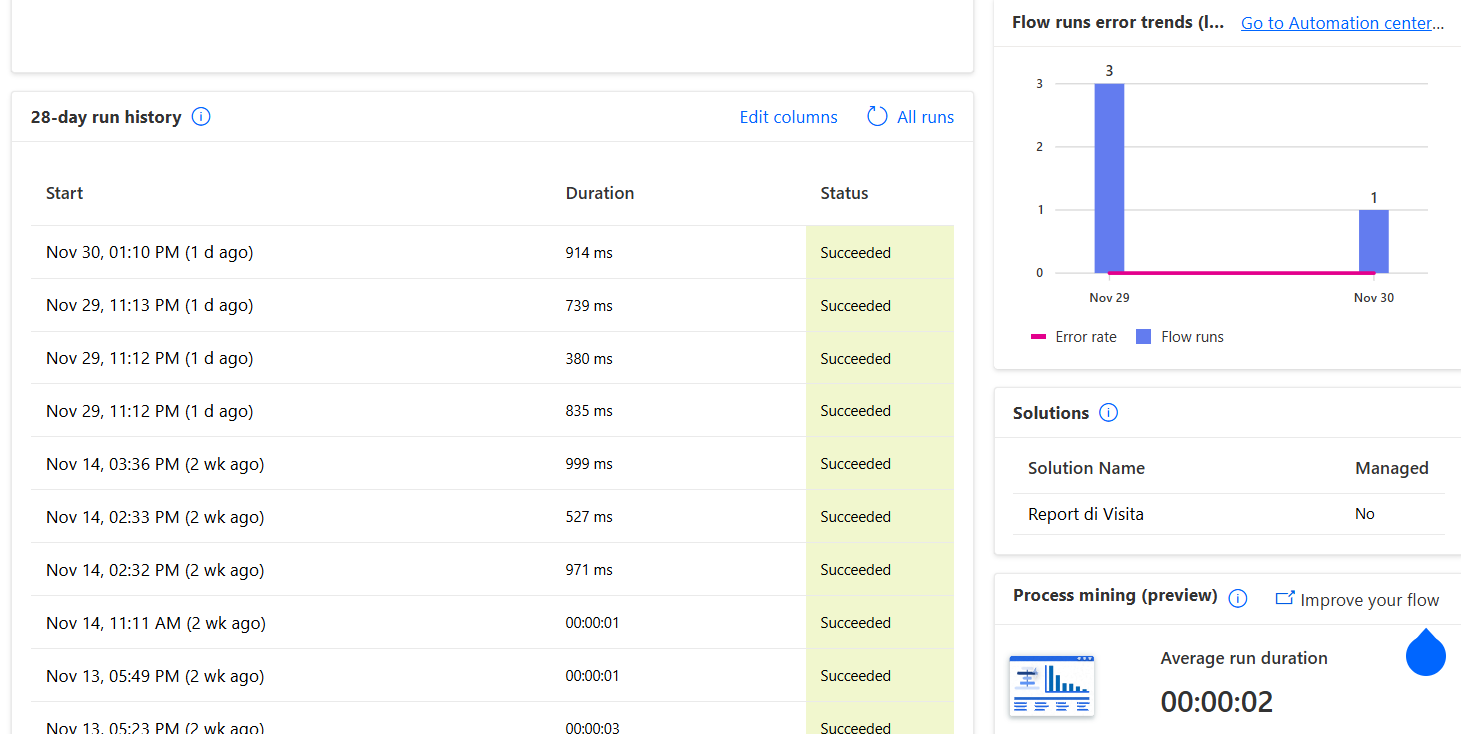
\includegraphics[width=1\columnwidth]{flowMonitor} 
    \caption{Vista parziale dell'interfacccia atta a monitorare un flusso.}
    \label{fig:flowMonitor}
\end{figure}

\newpage \subsection{Progettazione delle applicazioni aziendali}
Le attività di progettazione che ho svolto, relative alle applicazioni aziendali, sono state limitate alla scelta delle strategie da esplorare per risolvere i problemi emersi. Questo perché tali applicazioni erano già presenti da tempo al momento del mio arrivo in azienda.
Eccezione è fatta per l'applicazione "Non conformità" che, a differenza delle altre, era nelle sue prime fasi di sviluppo.\\
Al fine di comprenderne gli obiettivi ho preso parte a dei \emph{meeting} dedicati con il \emph{\emph{tutor}} aziendale e la parte del \emph{team} di sviluppo coinvolta.\\ 
Ho in seguito contribuito a progettare l'aspetto grafico e le soluzioni atte a soddisfarne i requisiti, ma il mio periodo di \emph{stage} è terminato prima che io potessi iniziare il loro sviluppo.  

\section{Codifica e documentazione}
In questa sezione sono presenti tutte le attività da me svolte al fine di sviluppare e implementare le soluzioni individuate in fase di progettazione.
\subsection{PoC iniziali}
Le prime fasi dello \emph{stage} sono state autonome e a supporto della comprensione ed esplorazione delle tecnologie a me richieste. 
Avendo iniziato le mie attività con Power Automate, ho realizzato un primo flusso al fine di testare l'utilizzo di: Trigger, Azioni, collegamento con i servizi Microsoft OneDrive ed Excel, Azioni condizionali, cicli Do until, inizializzazione e modifica di variabili.\\
Tale flusso viene eseguito automaticamente quando viene creato un \emph{file} dentro ad un \emph{path} specifico su OneDrive e di conseguenza invia un'approvazione notificata sia tramite Teams che Outlook.\\
Dopo aver ricevuto la risposta, il flusso agisce di conseguenza spostando il \emph{file} iniziale in un \emph{path} specifico in funzione dell'esito dell'approvazione. Viene in aggiunta eseguito un controllo sui \emph{file} già presenti nel percorso di destinazione e, nel caso fosse già presente un documento omonimo, il documento da spostare viene rinominato.\\
Questo controllo avviene ciclicamente incrementando un valore posto nel nome del \emph{file} fino al verificarsi dell'effettiva possibilità di eseguire lo spostamento.\\
Infine viene eseguito uno \emph{script} Excel il quale scrive in una tabella di \emph{log} le informazioni relative allo spostamento.
\begin{figure}[htbp] 
    \centering 
    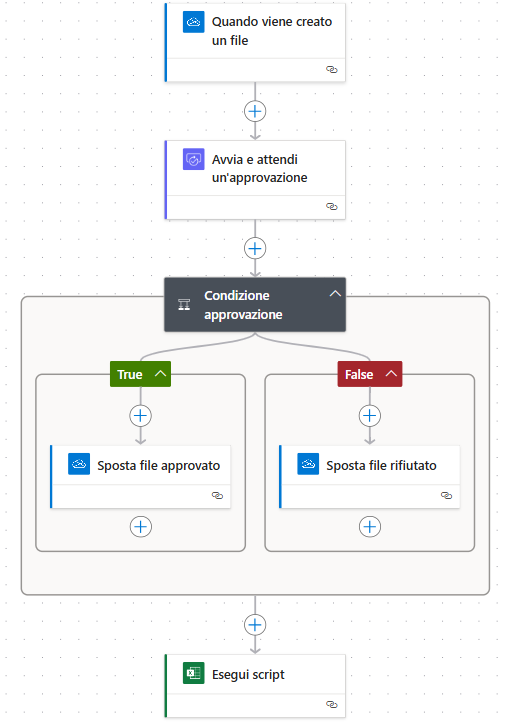
\includegraphics[width=0.5\columnwidth]{flussoApprovazioni} 
    \caption{Flusso per testare condizioni, approvazioni ed esecuzione di \emph{script}.}
    \label{fig:flussoApprovazioni}
\end{figure}
\newline \noindent A fini illustrativi l'immagine mostra una versione semplificata del flusso descritto. Essa esclude il controllo della presenza di un \emph{file} omonimo e quindi non include il ciclo Do until e l'inizializzazione e modifica di variabili.\\
Successivamente, ho prodotto una presentazione PowerPoint al fine di esporre al \emph{\emph{tutor}} aziendale le funzionalità, i lati positivi e i lati negativi delle tecnologie Power Automate e Power Apps, in funzione di quanto appreso durante la prima settimana di \emph{stage}.

\subsection{Sviluppo DevOps}
\label{Sviluppo DevOps}
\subsubsection*{Plan} 
Le attività pratiche legate alla fase di pianificazione sono la configurazione degli ambienti Planner e Taiga e la loro condivisione e utilizzo con i membri del \emph{team} coinvolti.\\
Inoltre, in collaborazione con lo stagista responsabile del progetto \hyperref[stageGiacomo]{Integrazione sistemi di pianificazione di progetto}, abbiamo esplorato la possibilità di integrare i flussi Power Automate al fine di sostituire le logiche, realizzate tramite complessi \emph{scirpt}, responsabili per l'interazione e la sincronizzazione tra le due piattaforme di pianificazione.\\
Per farlo abbiamo inoltre esplorato l'utilizzo dei \emph{webhooks}, ovvero degli strumenti \emph{web} che permettono di configurare l'invio automatico di chiamate \gls{http} di ritorno. Esse vengono eseguite da parte di un'applicazione \emph{web} al fine di permettere dell'utilizzatore di questo strumento di ricevere dati automaticamente al verificarsi di uno specifico evento.\\
A causa delle limitazioni incontrate nell'utilizzo di servizi di \emph{webhooks}, e della fine dello svolgimento dello \emph{stage} della persona con cui collaboravo, tali studi non hanno portato a soluzioni effettivamente utilizzate.

\subsubsection*{Code}
Le attività al fine di predisporre la fase Code, per la sua applicazione a progetti Power Automate e Power Apps, comprendono principalmente la realizzazione e la documentazione del sistema di versionamento individuato in fase di progettazione e la documentazione e l'applicazione degli strumenti per l'analisi statica del codice identificati.\\
Per il versionamento ho adattato, prima in un \emph{branch} di prova e poi nei restanti, il \emph{repository} Git dell'applicazione aziendale Report di visita in modo da rispecchiare le norme definite.
Esse riguardano le regole da seguire per versionare il progetto e la struttura dei percorsi dei \emph{file}, divisi in base alla loro funzione.\\  
Tali norme sono state definite con la collaborazione di parte del \emph{team} di sviluppo e dello stagista universitario responsabile del progetto \hyperref[stageDavide]{Applicativi di DevOps in ambito Sistemi}.\\ 
Per fare in modo di contenere nel \emph{repository} i \emph{file} relativi ai flussi Power Automate e le applicazioni Power Apps, è stata predisposta una cartella apposita al fine di contenere il pacchetto ZIP relativo alla Microsoft Solution del progetto.\\ 
Tale pacchetto nel \emph{repository} assume valore in ottica di \emph{backup} e ripristino, in caso sia necessaria l'esecuzione di una specifica versione del progetto.\\  
Per fare in modo che Power Apps riesca ad utilizzare la funzione integrata che gli permette di interfaccairsi con Git direttamente dalla sua interfaccia grafica, è necessario che nel \emph{repository} sia presente tale applicazione in un formato non compresso. È pertanto stato deciso di mantenere, per quanto ridondante, una copia dell'applicazione al fine di agevolare le fasi di sviluppo.\\ 
Per l'analisi statica del codice ho esplorato altri strumenti esterni come l'applicazione di strumenti di analisi statica consolidati, ad esempio SonarQube, applicati tramite IDE esterni ai dati generati da Power Automate e Power Apps.\\  
Inoltre ho constatato la possibilità di utilizzare gli strumenti diagnostici nativi di tali tecnologie anche tramite i comandi della Power Platform CLI, in modo da automatizzare la raccolta dei risultati.\\ 
Tuttavia, questa funzione risulta superflua, poiché i risultati sono più facilmente accessibili tramite l'interfaccia grafica durante le fasi di sviluppo. Inoltre, perde di utilità se, per verificare lo stato del codice, è necessario eseguire uno \emph{script} e analizzare un complesso \emph{file} JSON.\\ 
I documenti “Norme di progetto” e “Analisi statica” sono stati redatti e sono stati condivisi con il \emph{team} di sviluppo e con il \emph{\emph{tutor}} aziendale.\\  
Infine ho prodotto una presentazione PowerPoint contenente le principali informazioni presenti nei documenti citati e l'ho esposta al \emph{team} di sviluppo. 

\subsubsection*{Build}
Al fine di collegare il Job Jenkins con il \emph{repository}, senza dover utilizzare \emph{token} di accesso GitHub personali, ho utilizzato la funzione che permette di generare “GitHub Apps”. Esse sono applicazioni integrate in GitHub che permettono il collegamento tra i \emph{repository} desiderati con altri specifici strumenti e servizi, definendone con precisione il livello di accesso e autorizzazioni.  
\begin{figure}[htbp] 
    \centering 
    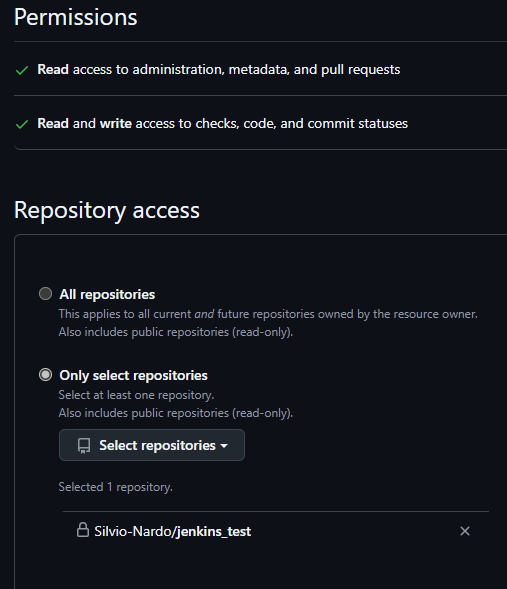
\includegraphics[width=0.4\columnwidth]{githubAppPermessi} 
    \caption{Configurazione dei permessi e selezione dei repository connessi ad una GitHub App.}
    \label{fig:githubAppPermessi}
\end{figure}
\newline Per automatizzare l'esportazione delle Microsoft Solutions e il loro caricamento nel \emph{repository}, ho adottato un Multibranch Pipeline Job Jenkins. Il relativo Jenkinsfile da me prodotto esegue, tramite i propri Stage, le seguenti operazioni:
\begin{itemize}
    \item Seleziona il corretto \emph{branch} del \emph{repository} ed esegue un comando \emph{pull}
    \item Cerca modifiche nella cartella relativa all'applicazione Power Apps
    \item Esegue l'autenticazione Micorsoft tramite gli appositi comandi forniti dalla Power Platform CLI
    \item Esporta la Microsoft Solutions
    \item Controlla l'eventuale presenza di una omonima Solution già presente nel \emph{repository} e, se presente, la elimina 
    \item Carica il pacchetto relativo alla nuova versione della Solution nel \emph{repository}
\end{itemize}
Ho redatto il documento “Guida Jenkins”, il quale comprende tutte le nozioni e le norme relative all'adozione di Jenkins, al fine di applicare la fase Build ai progetti Power Automate e Power Apps e l'ho condiviso con il \emph{team} di sviluppo e con il \emph{\emph{tutor}} aziendale.

\subsubsection*{Test}
\label{testProgrammazione}
L'applicazione di \emph{test} automatici per i flussi Power Automate è avvenuta, oltre all'utilizzo degli strumenti nativi già discussi, tramite lo sviluppo di soluzioni esterne sfruttando le chiamate \gls{http}.
Esse permettono la comunicazione e lo scambio di dati tra flussi Power Automate e altri flussi o applicazioni: esiste infatti la possibilità di richiamare lo specifico Trigger “Alla ricezione di una richiesta HTTP”, il quale genera un personale URL (Uniform Resource Locator), ovvero una sequenza di caratteri che identifica univocamente l'indirizzo di una risorsa su una rete di \emph{computer}.\\
In seguito è possibile utilizzare la corrispondente azione “Response” al fine di rispondere al chiamante con l'\emph{output} della richiesta.\\
\begin{figure}[htbp] 
    \centering 
    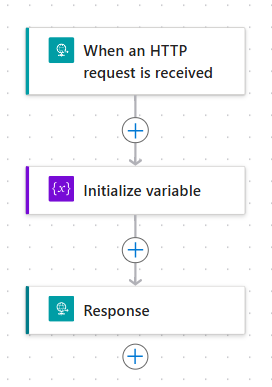
\includegraphics[width=0.3\columnwidth]{flussoHttp} 
    \caption{Flusso di esempio per ricevere e risondere a chiamate HTTP.}
    \label{fig:flussoHttp}
\end{figure}
\newline L'invio delle chiamate e l'analisi dei dati di \emph{output} inviati dal flusso oggetto di \emph{test}, sono avvenute mediante uno \emph{script} Node.js con l'ausilio della libreria “Axios”, la quale offre funzionalità per l'invio e la ricezione asincrona delle chiamate \gls{http}.\\
Per poter inviare una chiamata al flusso desiderato tramite \emph{script}, è necessario ottenere, tramite un'ulteriore chiamata \gls{http}, un \emph{token} Microsoft di autenticazione.
\begin{figure}[htbp] 
    \centering 
    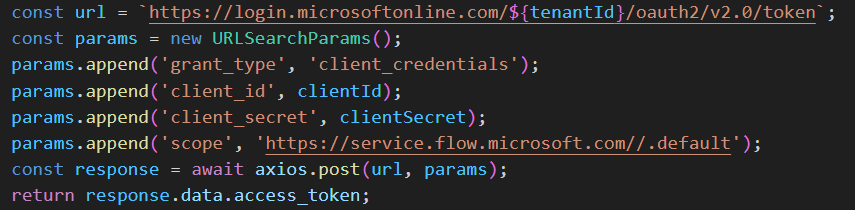
\includegraphics[width=0.8\columnwidth]{richiestaTokenNode} 
    \caption{Parte dello \emph{script} responsabile per l'ottenimento del \emph{token} di autenticazione.}
    \label{fig:richiestaTokenNode}
\end{figure}
\newline In seguito è possibile, aggiungendo l'\emph{output} ottenuto dalla precedente chiamata, inviare la richiesta di esecuzione al flusso da testare.\\
Grazie all'Azione del flusso “Response”, lo \emph{script} può proseguire alla ricezione della risposta contenente l'\emph{output} di Power Automate, in modo da analizzarla e determinarne l'esito.
\begin{figure}[htbp] 
    \centering 
    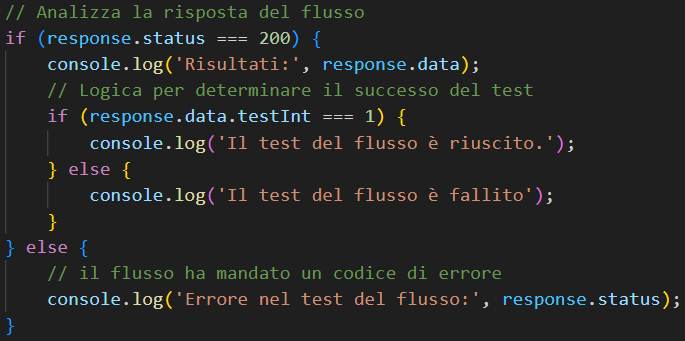
\includegraphics[width=0.6\columnwidth]{analisiEsitoTest} 
    \caption{Parte dello \emph{script} responsabile per l'analisi dell'esito dei \emph{test} su flussi Power Automate.}
    \label{fig:analisiEsitoTest}
\end{figure}
\newline Nell'immagine è mostrata una porzione dello \emph{script} nel quale viene, a fini dimostrativi, controllato se il risultato della chiamata è stata un successo, definito con codice 200, e se l'\emph{output} del flusso è uguale ad un intero di valore 1. In funzione dell'esito del controllo e dello stato di successo della chiamata, viene mostrato a schermo un relativo messaggio.\\
Ai fini di rendere automatico questo processo, l'esecuzione dello \emph{script} illustrato è stato incluso nel Jenkinsfile relativo al Job Jenkins dell'applicazione aziendale Report di visita.
Tale pratica garantisce la qualità e la funzionalità attesa dai flussi testati, però è da considerare che la natura dei prodotti realizzati con Power Automate richiede che essi vengano modificati, al fine di essere predisposti alla ricezione e alla risposta delle chiamate \gls{http} di \emph{test}. Inoltre è da tenere in considerazione che tali funzioni necessitano della licenza \emph{premium}.\\\\
Per le applicazioni Power Apps ho esplorato la possibilità di estrarre, tramite la funzione “Scarica suite”, un \emph{file} contenente le azioni registrate dallo strumento Test Studio ma, in funzione delle conclusioni esplicitate precedentemente riguardo tale strumento, la strategia non è stata integrata nel sistema di \emph{testing}.\\\\
Ho prodotto il documento “Test dinamici”, contenente tutte le informazioni relative ai metodi individuati per effettuare tali \emph{test} su Power Automate e su Power Apps, sia con strumenti nativi che esterni. Ho aggiornato il documento “Guida Jenkins” al fine di contenerne anche le nozioni riguardanti quanto descritto.\\
Tali documenti sono stati condivisi con il \emph{team} di sviluppo e con il \emph{\emph{tutor}} aziendale.\\
Inoltre ho prodotto, ed esposto al \emph{team} di sviluppo, una presentazione PowerPoint contenente le principali informazioni apprese e le soluzioni individuate e sviluppate relativamente alle fasi Build e Test. 

\subsubsection*{Deploy}
Al fine di comprendere e testare l'applicazione della fase Deploy ho esplorato, insieme a parte del \emph{team} di sviluppo, le funzionalità legate all'importazione delle Microsoft Solutions, gestite e non gestite, all'interno di diversi ambienti di produzione.\\ 
Al fine di agevolare il collegamento agli \emph{account} e ai servizi Microsoft corrispondenti al nuovo ambiente, sono state utilizzate, ed inserite all'interno della relativa Solution, i “riferimenti alle connessioni”. Essi sono entità che rappresentano il collegamento tra un'applicazione, un servizio o un flusso e una risorsa esterna, e offrono la possibilità di essere cambiati in maniera dinamica durante la fase di importazione in un ambiente.\\\\
L'applicazione delle fasi di \gls{DevOps} Release, Operate e Monitor, a seguito delle attività di analisi e progettazione, non hanno avuto necessità di attività di sviluppo aggiuntive. 

\subsection{Attività sulle applicazioni aziendali}
\label{sviluppoApplicazioni}
\subsubsection*{Report di visita}
Le attività di sviluppo dell'applicazione aziendale Report di visita hanno affiancato le attività di ricerca del mio \emph{stage} per la maggior parte della sua durata.\\
Esse, oltre all'integrazione delle pratiche \gls{DevOps} descritte precedentemente, si sono focalizzate sulle strategie di \emph{retrieve} dei dati tramite appositi flussi Power Automate collegati all'applicazione.\\
Lo strumento di archiviazione utilizzato principalmente è stato SharePoint, ma è stata testata anche la possibilità \emph{premium} di leggere dati da SQL Server.\\
Le principali difficoltà affrontate sono relative ai limiti sul numero di \emph{record} ottenibili per ogni richiesta a SharePoint:
\begin{itemize}
    \item Essendo per Power Apps una funzione non delegabile, ovvero che non può delegare l'elaborazione dei dati al \emph{server}, è presente il limite di 500 \emph{record} ottenibili di \emph{default} estendibile fino a 2000 modificando le impostazioni. Inoltre eventuali filtri sulla ricerca vengono applicati solo dopo aver ricevuto quel numero di dati, pertanto, il risultato ottenuto è un insieme limitato del risultato atteso.
    \item Eseguendo l'analoga funzione da un flusso Power Automate, si incorre in un ulteriore limite imposto da Sharepoint uguale a 5000 risultati ottenibili per chiamata.\\
    In merito sono state esplorate soluzioni legate al precaricamento di tutti i dati, mediante chiamate multiple, al fine di applicare successivamente il filtraggio dei dati richiesti, e all'utilizzo di chiamate \gls{http} a servizi SharePoint. Queste soluzioni sono state successivamente scartate a causa degli eccessivi tempi di esecuzione e ad altre limitazioni incontrate, come l'impossibilità per SarePoint di eseguire il comando di ricerca per sottostringa.
    \item Dopo aver ottenuto i dati desiderati, sfruttando particolari funzionalità di indicizzazione delle liste SharePoint, sono state incontrate difficoltà legate all'aggiornamento grafico di alcuni componenti fondamentali dell'applicazione utilizzati per mostrare dinamicamente i contenuti ricavati.\\
    Tale problema è stato risolto tramite lo sviluppo di un nuovo componente \emph{custom}.  
\end{itemize}
Al fine di fare \emph{test} su liste SharePoint, popolate dinamicamente da un numero elevato di elementi, ho generato tabelle Excel in maniera automatica scrivendo appositamente degli “Office Scripts”.\\
Le mie attività di sviluppo legate alle applicazioni Registro accessi e "Non conformità" sono legate ad aspetti grafici e all'individuazione di possibili risoluzioni di problemi legati alle singole funzioni Fx. 

\subsection{Attività con Angular}
Al fine di comprendere il funzionamento e lo sviluppo di progetti basati su Angular, ho realizzato una basilare applicazione \emph{web} che mostrava nell'interfaccia grafica immagini e testo.\\
Essa è stata il punto di partenza per lo sviluppo di una \emph{suite} di \emph{test} eseguiti con l'apposito strumento “Karma”. Tale esecuzione è poi stata automatizzata in un Job Jenkins di tipo \emph{pipeline}, il quale: 
\begin{itemize}
    \item Seleziona e utilizza la versione di Node.js predeterminata
    \item Preleva il progetto dal \emph{repository} Git
    \item Esegue i \emph{test} di unità definiti
    \item Compila i \emph{file} e genera il relativo pacchetto composto da elementi HTML e JavaScript
    \item Mostra a schermo il risultato dei \emph{test} in un apposito grafico
    \item Salva gli artefatti creati in Jenkins, vincolando la presenza dei salvataggi ai soli tre più recenti
    \item Pulisce il \emph{workspace} relativo al Job e alle compilazioni avvenute  
\end{itemize}
\begin{figure}[htbp] 
    \centering 
    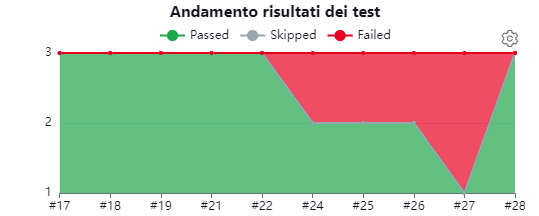
\includegraphics[width=0.7\columnwidth]{graficoTest} 
    \caption{Grafico dell'esito dei \emph{test} generato da Jenkins.}
    \label{fig:graficoTest}
\end{figure}
Inoltre ho applicato quanto appreso per produrre un ulteriore \emph{pipeline} Job al fine di replicare le fasi di \gls{DevOps} anche su progetti aziendali realizzati con Angular.\\
Infine ho generato il documento “Angular in Jenkins” contenente quanto affrontato in merito e l'ho esposto al \emph{team} di sviluppo e al \emph{\emph{tutor}} aziendale. 

\section{Risultati raggiunti}
\subsection{Risultati qualitativi}
Lo studio delle tecnologie Power Automate e Power Apps ha fatto emergere la loro natura: essi sono \emph{software} utili nei casi in cui si debba realizzare un'applicazione semplice rapidamente, ma è da considerare che sono strumenti ancora relativamente nuovi, quindi privi di una documentazione esaustiva e aventi \emph{features} soggette a frequenti e importanti modifiche.\\
Offrono la possibilità di connettersi agevolmente con i servizi Microsoft ma presentano allo stesso tempo un alto numero di limitazioni, le quali non offrono la libertà di sviluppo ottenibile con i consolidati strumenti e linguaggi di programmazione.\\ 
Lo studio da me svolto durante lo \emph{stage} ha fatto emergere l'effettiva possibilità di applicare le metodologie \gls{DevOps} a progetti realizzati con Power Auotmate e Power Apps.\\\\
Tramite periodi di sviluppo collaborativo, ho dimostrato la possibilità di applicare strategie di collaborazione e condivisione delle risorse tra membri del \emph{team} di sviluppo.\\ 
Ho definito le norme di versionamento che il \emph{team} deve seguire per organizzare efficacemente tutte le parti che compongono un progetto Power Automate/Power Apps, testando la possibilità di effettuare il ripristino di specifiche versioni rilasciate.\\ 
Ho applicato metodologie di analisi statica del codice e \emph{testing} dinamico, sia mediante strumenti nativi che esterni, al fine di verificare il corretto funzionamento e garantire la qualità dei prodotti realizzati.\\ 
Ho dimostrato la possibilità di gestire il ciclo di vita del \emph{software} prodotto, relativamente alle tecnologie in oggetto, comprese le fasi di distribuzione dei prodotti e il loro monitoraggio.\\ 
Ogni nozione da me acquisita, ogni norma stipulata e ogni soluzione implementata è stata documentata ed è stata resa disponibile al personale attraverso gli strumenti di condivisione aziendale. 

\subsection{Risultati qualitativi}
\begingroup
\renewcommand\arraystretch{1.3}
\begin{longtable}{|p{11cm}|}
    \caption{Documenti che ho prodotto durante lo \emph{stage}.}
    \label{tab:risultatiQualitativi}\\
    \hline \multicolumn{1}{|c|}{\textbf{Documenti prodotti}}\\ \hline \endfirsthead
    \hline \multicolumn{1}{|c|}{\textbf{Documenti prodotti}}\\ \hline \endhead
    \hline \endhead
    \hline \endfoot
    \hline \endlastfoot
    \hline “Analisi statica del codice”\\
    \hline “Norme di versionamento”\\
    \hline “Test dinamici”\\
    \hline “Guida Jenkins”\\
    \hline “Angular in Jenkins”\\
    \hline Presentazione sulle funzionalità, i lati positivi e i lati negativi di Power Automate e Power Apps\\
    \hline Presentazione relativa alle limitazioni di tali tecnologie e le rispettive soluzioni individuate\\
    \hline Presentazione relativa al versionamento e all'analisi statica del codice\\
    \hline Presentazione relativa ai processi Build e ai \emph{test} dinamici\\
    \hline Presentazione finale realizzata in collaborazione con gli altri stagisti universitari riguardo a quanto fatto durante i nostri \emph{stage}\\
\end{longtable}
\endgroup
 
\subsection{Risultati quantitativi}
\begingroup
\renewcommand\arraystretch{1.3}
\begin{longtable}{|p{11cm}|}
    \caption{Software che ho prodotto durante lo \emph{stage}.}
    \label{tab:risultatiQuantitativi}\\
    \hline \multicolumn{1}{|c|}{\textbf{Software prodotti}}\\ \hline \endfirsthead
    \hline \multicolumn{1}{|c|}{\textbf{Software prodotti}}\\ \hline \endhead
    \hline \endfoot
    \hline \endlastfoot
    \hline PoC sui flussi approvativi\\
    \hline PoC sull'integrazione di chiamate \gls{http} con i flussi\\
    \hline Jenkinsfile per progetti Power Automate/Power Apps\\
    \hline \emph{Script} Excel per la creazione automatica di tabelle\\
    \hline \emph{Script} Node.js per il \emph{test} di flussi tramite chiamate \gls{http}\\
    \hline Sviluppo di funzioni Fx sul prodotto aziendale Report di visita\\
    \hline Flussi per il \emph{retreive} dei dati da liste SharePoint\\
    \hline Progetto di esempio Angular\\
    \hline Jenkinsfile relativo al progetto di esempio Angular\\
\end{longtable}
\endgroup

